\chapter{Design and test specification} \label{ch:req}
This chapter elaborates on the requirements for the system and derives a test specification which will describe how to test for the requirements.\\

A way to identify the performance of a design using different design metrics is the cost function. The cost function specifies the overall cost of a design and is a function of the different design metrics:
\begin{equation}
C = f(A,T,P,N,S) = a_1\cdot A + a_2 \cdot T + a_3 \cdot P + a_4 \cdot N + a_5 \cdot S
\end{equation}
where $A$ is area, $T$ is time, $P$ is power, $N$ is numerical properties, $S$ is the stereo matching result from Middlebury test and $a_i$ tells the importance of the associated metric.\\
It is the task of the system designer to minimize this cost. And due to $a_i$ the cost function can be changed to fit the priorities of the application.\\

For this thesis, the number one priority is the time metric since it is required that the algorithm should be executable in real-time. The stereo matching metric is also important since it describes the quality of the resulting disparity map i.e. the number false disparity values. Numerical properties are 3rd most important metric since this can affect the result from the algorithm since the cost value may have added noise. Area is not as important because if the target FPGA is too small then HSA Systems will use a larger FPGA but larger area often equals more expensive hardware. Power is not important either since the stereo setup is intended as a part of industrial systems hence power is easily accessible.\\

An ordered list of priorities for the design metrics in this project:
\begin{multicols}{2}
  \begin{enumerate}
    \item Time
    \item Stereo matching result
    \item Numerical properties
    \item Area 
    \item Power\\~\\
  \end{enumerate}
\end{multicols}

In this thesis, the cost function will be used when e.g comparing the different algorithms found in chapter \vref{ch:alganalysis}.

\section{Requirement specification}
This section will contain a table with the requirements for the system. Each parameter will be given a number, a value which should be met, the unit for the value, additional information for the requirement and a reference to where the discussion for the requirement can be found.
\begin{table}[ht!]
  \centering
  \begin{tabular}{l m{2cm} c c m{5cm} m{1.9cm}}
  \toprule
  \textbf{No.} & \textbf{Parameter} & \textbf{Value} & \textbf{Unit} & \textbf{Additional Information} & \textbf{Source} \\
  \midrule
  1 & Frame rate & $\geq 10$ & fps & & Section \vref{req:framerate} \\
  \midrule
  2 & Disparity precision & $\leq 5$ & \si{\milli\meter} & \tabitem Either directly or using \newline \hspace*{0.4cm}subpixel refinement \newline \tabitem In the range 0.5-\SI{1.5}{\meter}  & Section \vref{req:dispre}\\
  \midrule
  3 & Camera resolution & 2464$\times$2056 & pixels & & Section \vref{req:camres} \\
  \midrule
  4 & Pixel size & \num{3.45} & \si{\micro\meter} & & Section \vref{req:pixelsize} \\  
  \midrule
  5 & Focal length & \num{7.09} & \si{\milli\meter} & & Section \vref{req:focallen} \\
  \midrule
  6 & Scene size & \num{1.5}$\times$\num{1.5} & \si{\meter} & & Section \vref{req:scenesize} \\
  \toprule
  \multicolumn{6}{l}{The algorithm should be implemented on a \textit{Xilinx Zynq Z7020}}\\
  \bottomrule
  \end{tabular}
\end{table}

\section{Test specification}
This section will describe how the system can be tested in order to ensure that the requirements are fulfilled. \\

Requirement 1: frame rate can be tested by running the finalized implementation and measure the runtime which should be \SI{\leq 100}{\milli\second}. \\

Requirement 2: disparity precision. This requirement can be tested if a working stereo camera setup is developed. \\
HSA Systems has produced a depth precision test object with small depth differences. The object is shown on figure \vref{fig:3dpreobj}. The object consists of five sets of steps with each stair having different depth increment. Looking at \vref{fig:3dpretestpic} the set of steps at the bottom have a depth difference of \SI{5}{\milli\meter} between each step. The set of steps just above have a depth difference of \SI{4}{\milli\meter} between each step. This pattern continues and results in the top set of steps to have a depth difference of \SI{1}{\milli\meter}. The small shapes in the middle of each step have a depth difference of \SI{0.5}{\milli\meter} alternately protrude from or recess into the steps.\\

\begin{figure}[ht]
  \centering
  \begin{subfigure}[t]{0.45\textwidth}
    \centering\raisebox{22.25mm}{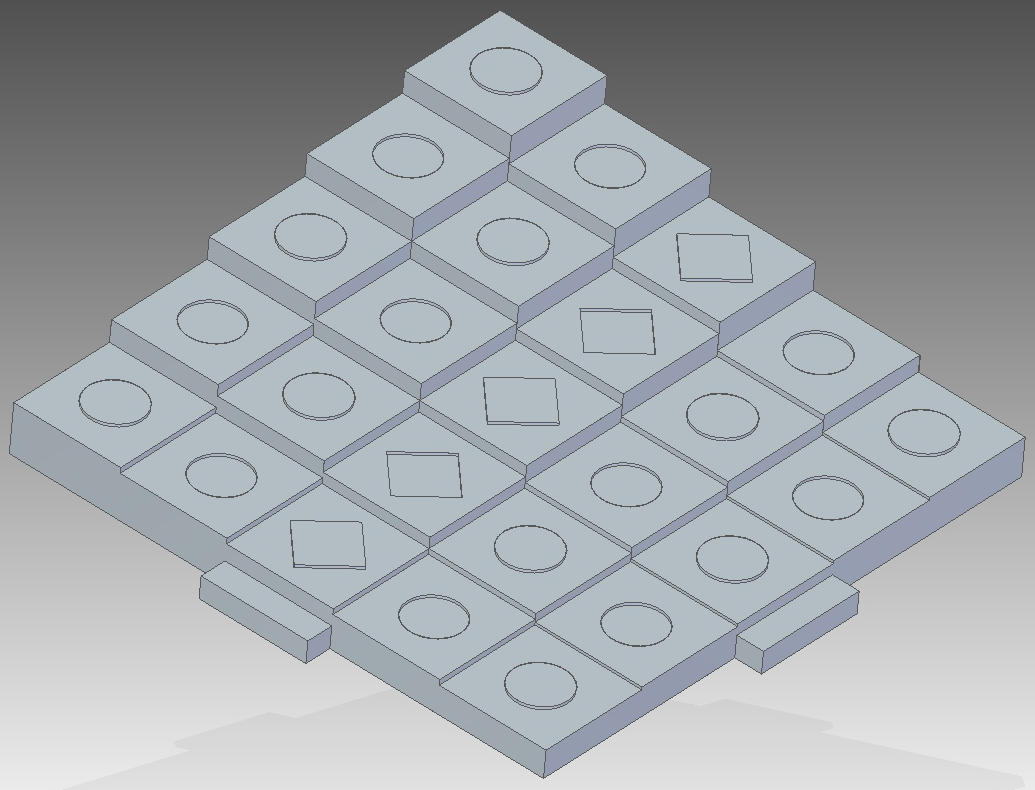
\includegraphics[width=0.9\textwidth]{figures/3dprecisiontest}}
    \caption{3D model of depth precision test object}
    \label{fig:3dpretest}
  \end{subfigure}\hspace{0.5cm}
  \begin{subfigure}[t]{0.45\textwidth}
    \centering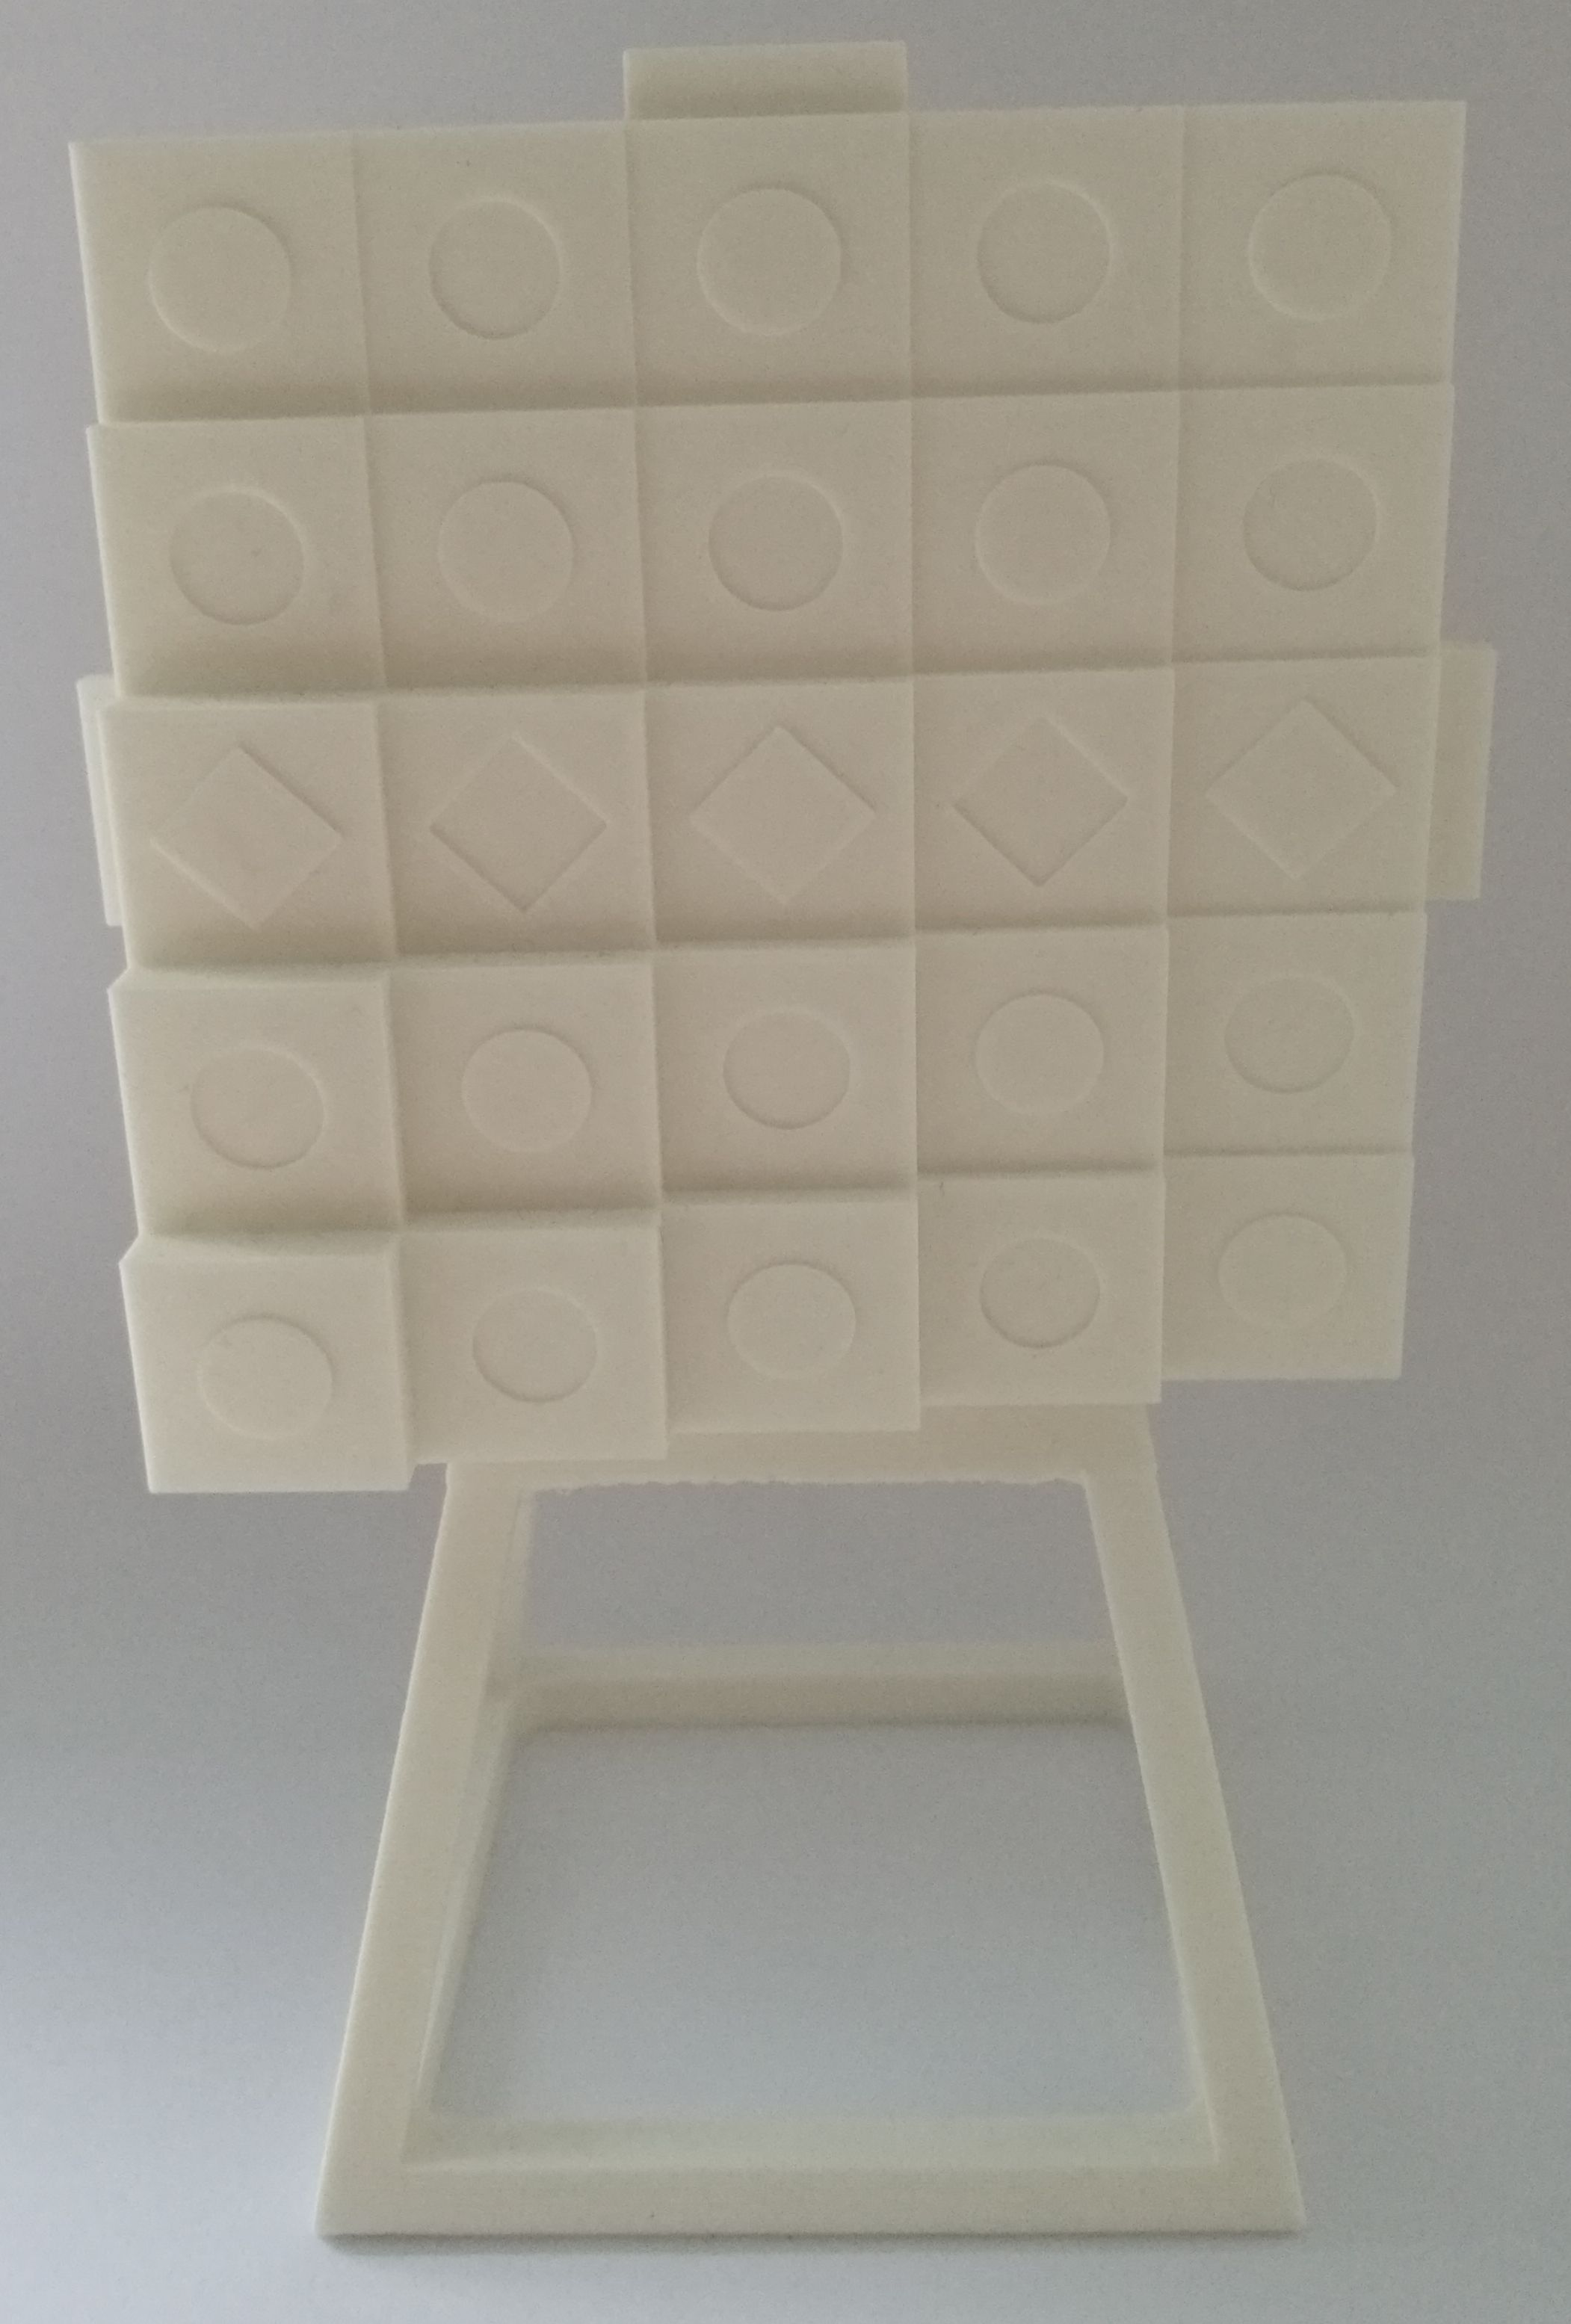
\includegraphics[width=0.9\textwidth]{figures/testobject_foot}
    \caption{Picture of 3D printed depth precision test object}
    \label{fig:3dpretestpic}
  \end{subfigure}
  \caption{Depth precision test object \label{fig:3dpreobj}}
\end{figure}
Placing this object at a specific distance the depth precision can be tested. If the steps in lowest set of steps can be distinguished from each other in the disparity map then the depth precision is \SI{\leq 5}{\milli\meter}.\\
If the implementation can distinguish between the lowest set of steps and the object is placed at \SI{1.5}{\meter} from the camera setup then the requirement is fulfilled. The rest of the steps help determine if the camera have a better precision than required.\\
The Middlebury test set does not contain images where specific areas contain depth increments of 2 mm and therefore these images can not be used for testing this requirement and calculations \vref{sec:disppre} are used instead.\\

Requirement 3: camera resolution is fulfilled by choosing the correct camera hardware but is essential to be fulfilled for requirement 2 to be fulfilled.\\

requirement 4: pixel size is fulfilled by choosing the correct camera hardware but is essential to be fulfilled for requirement 2 to be fulfilled.\\

requirement 5: focal length is fulfilled by choosing the correct camera hardware but is essential to be fulfilled for requirement 2 to be fulfilled.\\

Chapter \vref{ch:acctest} will perform the available tests.
